\chapter{Analýza}
V tejto kapitole sa pozrieme na zopár problémov a ich riešení, na ktoré sme narazili počas vytvárania nášho analyzátoru.
Ako prvé sme sa museli rozhodnúť v akom jazyku budeme náš projekt implementovať. Na to si autor zvolil obecne rozšírený jazyk C++, pretože ho pozná najlepšie a má s ním najviac skúseností. Táto voľba nás zároveň v ničom zásadne neobmedzila a nemala negatívny dopad na celkový výsledok aplikácie. Teraz sa pozrieme na niekoľko konkrétnych problémov a spôsoby akými sme ich vyriešili.

\section{Získanie USB packetov}
Na získavanie USB paketov nám bude obecne slúžiť paket sniffer. Väčšina paket analyzátorov má implementované vlastné sniffery a preto sme sa o to pokúsili tiež. Narazili sme ale na niekoľko zásadných problémov, ktoré sa úzko viažu s platformou na ktorú cielime s našou aplikáciou~--~Windows.

V minulej kapitole~\ref{kap02:sec:hid_arch} sme opisovali stavbu HID zariadení vo windowse, čím sme sa dozvedeli, že device stack každého z nich je postavený na \textit{hidclass.sys}. Microsoft dokumentácia podrobnejšie opisuje komunikáciu medzi HID zaridením a kernel/user-mode aplikáciou~\cite{hid_opening_collections} za pomoci API tohoto driveru -- \textit{HID API}~\cite{hid_api}.
Pri tejto komunikácii sme schopní zachytiť USB pakety posielané zariadením a neskôr ich analyzovať. Keďže naša aplikácia beží v user-mode, prejdeme si práve tento spôsob komunikácie:
\begin{enumerate}
\item Aplikácia nájde a identifikuje HID zariadenie.
\item Aplikácia pomocou metódy \texttt{CreateFile} otvorí spojenie s HID zariadením.
\item Aplikácia pomocou \textit{HID API} metód \texttt{HidD\_Xxx} získa \textit{Preparsed Data} a informácie ohľadom HID zariadenia.
\item \label{kap03:read:paket} \textbf{Aplikácia použije metódu \texttt{ReadFile} resp. \texttt{WriteFile} na získanie inputu zariadenia resp. poslanie reportu zariadeniu.}
\item Aplikácia pomocou \textit{HID API} metód \texttt{HidP\_Xxx} interpretuje HID reporty.
\end{enumerate}

Podstatný je práve bod~\ref{kap03:read:paket} v ktorom vidíme, že pomocou metódy \texttt{ReadFile} sme schopní od daného zariadenia získať USB pakety, ktoré reprezentujú jeho input. Tie by sme následne mohli pomocou nášho analyzátoru spracovať. Tu narážame na prvý problém, ktorý sa priamo viaže na platformu Windows a ktorý si detailnejšie opíšeme v nasledujúcej sekcii.

\subsection*{Windows exclusive mód}
Windows má definovaný tzv. \textit{Access Mode}, ktorý určuje restrikciu prístupu \textit{HID Clienta} k HID zariadeniu. 
Ten môže byť buď \textit{Shared} alebo \textit{Exclusive}. \textit{Exclusive Mode} zabraňuje ostatným \textit{HID Clientom} v zachytávaní alebo získavaní inputu HID zariadenia, pokiaľ nie sú hlavným príjemcom daného inputu. Preto z bezpečnostných dôvodov otvára \textit{RIM (Raw Input Manager)} niektoré zariadenia v \textit{Exclusive Mode}.

Ak je zariadenie otvorené v \textit{Exclusive Mode}, aplikácia má stále prístup k niektorým jeho údajom pomocou  \textit{HID API}~\cite{hid_api} metód  \texttt{HidD\_\textbf{Get}Xxx}. Tieto metódy nám obecne umožnia získať niektoré descriptory zariadenia, tak ako aj jeho \textit{Preparsed Data}. Nie je nám ale umožnené volať metódu \texttt{ReadFile}, takže nemáme akým spôsobom zachytávať komunikáciu HID zariadenia s clientom.

Tabuľka zariadení~\cite{hid_access} (obrázok~\ref{obr:kap3:access_mode}), ktoré \textit{RIM} otvára v \textit{Exclusive Mode} obsahuje aj tie, ktoré sme si v úvode zvolili ako podmnožinu HID zariadení na analýzu -- myš a klávesnica.

\begin{figure}[!htb]
	\centering
	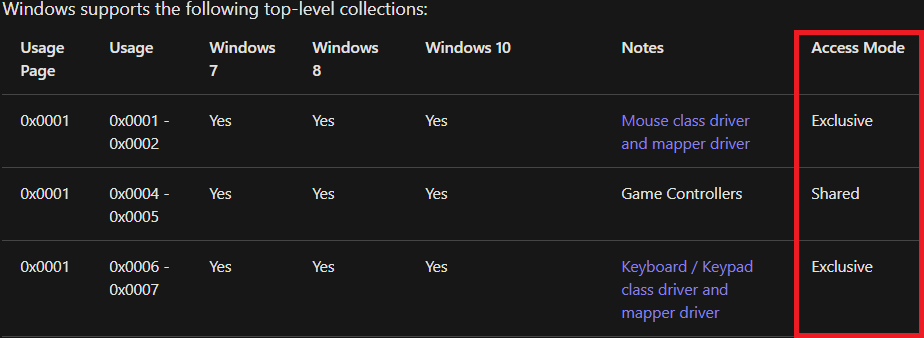
\includegraphics[width=\textwidth]{img/kap3_access_mode}
	\caption{Tabuľka zariadenía ich \textit{Access Mode}. Zariadenia postupne po riadkoch -- myš, joystick a klávesnica}
	\label{obr:kap3:access_mode}
\end{figure}

\subsection*{Známe knižnice}
Keďže komunikáciu nemôžeme zachytávať priamo pomocou \textit{HID API}~\cite{hid_api} metód, rozhodli sme sa skúsiť použiť niektoré známe knižnice na sledovanie USB zbernice. 

Pravdepodobne najznámejšou z nich je \textit{libusb}~\cite{libusb} -- knižnica napísaná v jazyku C, ktorá slúži na poskytnutie prístupu k USB zariadeniu. Je cielená na programátorov aby im uľahčila vývoj aplikácií, ktoré komunikujú s USB hardwarom. Podporuje viaceré platformy, medzi ktorými sa nachádza aj Windows. Zároveň beží v user-mode, takže aplikácia ktorá ju využíva nepotrebuje žiadne špeciálne privilégiá na používanie \textit{libusb API}. Ďalšou výhodou je, že podporuje všetky verzie USB od 1.0 až po 3.1. Je schopná zachytiť všetky typy prenosov (control,bulk,interrrupt,isochronus), a teda by sme pomocou nej mohli sledovať celú komunikáciu so zariadením vrátane počiatočného nakonfigurovania. Bohužiaľ, ani pomocou tejto knižnice sme neboli schopní získať prístup k zariadeniam, ktoré Windows otvára v exclusive móde.

Keďže sa zameriavame na HID zariadenia, skúsili sme hľadať niečo viac špecifické práve pre túto triedu USB zariadení -- to nás zaviedlo k \textit{HIDAPI}~\cite{hidapi_library}. \textit{HIDAPI} je ďalšia veľmi rozšírená knižnica, ktorá umožňuje komunikáciu s USB zariadeniami z HID triedy a takisto beží na viacerých patformách vrátane Windowsu. Pretrváva tu ale rovnaký problém ako s minulou knižnicou -- nie je možné získať prístup k zariadeniam, ktoré sú otvorené vo Windows exclusive móde.

Keďže sme nevedeli získať input zariadenia pomocou \textit{hidclass.sys} driveru a ani pomocu iných third-party aplikácií, skúsime sa pozrieť či nemáme k dispozícii filter driver, ktorý by nám poskytol prístup k inputu daného zariadenia.

\subsection*{Filter Driver}
Windows ponúka niekoľko vstavaných driverov pre rôzne typy zariadení. Konkrétne pre myš a klávesnicu windows ponúka 2 filter drivery -- \textit{Moufiltr}~\cite{moufiltr} (upper-level filter driver pre myš) a \textit{Kbfiltr}~\cite{kbfiltr} (upper-level filter driver pre klávesnicu). Tie ale podporujú len legacy zariadenia -- non-USB, non-Bluetooth a non-I2C zariadenia.

Riešením by teda bolo naprogramovanie vlastného filter driveru pre myš a klávesnicu. Toto je ale už nad rámec našej práce a preto upustíme od myšlienky implementácie vlastného USB snifferu a použijeme už existujúcu third-party aplikáciu.

\subsection*{Third-party aplikácie}
\label{kap03:third_party}
Na zachytávanie USB paketov sme sa rozhodli použiť \textit{USBPcap}~\cite{usbpcap}, s ktorým sme sa už stretli v kapitole~\ref{uvod:sec:Wireshark} keď sme opisovali Wireshark a rôzne sniffery, s ktorými je schopný spolupracovať. USBPcap je veľmi rozšírený Windows sniffer USB paketov a jeho hlavnou výhodou je jednoduchá inštalácia. Takisto nám vyhovuje, že je s ním schopný spolupracovať Wireshark, čo nám častokrát počas vývoja poskytlo spôsob akým sme si mohli overiť správnosť nami vykonanej analýzy niektorých paketov. Daný sniffer zachytáva pakety do súborov v obecne známom formáte pcap~\cite{pcap}. 

Miernou nevýhodou je, že nepodporuje čítanie zo súboru do ktorého práve zapisuje -- analýzu paketov v reálnom čase tak budeme musieť vykonať trochu iným spôsobom, a to za pomoci Wiresharku. Ako sme už spomínali, Wireshark je schopný spolupráce s USBPcapom a zároveň podporuje ukladať výstup analýzy do súboru, ktorý je takisto formátu pcap. Wireshark už ale podporuje čítanie z daného súboru počas toho ako do neho zapisuje. To znamená, že ak budeme chcieť vykonať analýzu v reálnom čase, urobíme to pomocou Wiresharku (konkrétnejší postup si ukážeme neskôr v užívateľskej dokumentácii v kapitole~\ref{udok:chap}).



\section{Sémantická analýza dát}
Ako sme už naznačili v kapitole~\ref{uvod:sec:HID}, na vykonanie sémantickej analýzy inputu HID zariadenia je potrebné získať informácie o danom inpute z Report Descriptoru konkrétneho zariadenia. V tejto kapitole si vysvetlíme formát Report Descriptoru a ako nám informácie ktoré reprezentuje pomôžu v sémantickej analýze inputu HID zariadenia.

\subsection*{Report Descriptor}
\label{kap03:sec:report_desc}
Celková štruktúra Report Descriptoru je opísaná v HID Class Specification~\cite{report_desc}. Descriptor sa skladá z tzv. itemov, ktoré obsahujú informácie o danom zariadení. Každý item obsahuje hlavičku, ktorá sa skladá z troch častí:
\begin{itemize}
\item Typ
\item Tag
\item Veľkosť
\end{itemize}

Existujú 3 typy itemov : \textit{Main}, \textit{Global} a \textit{Local}. Main item udáva informácie o konkrétnej časti zariadenia (napríklad o tlačidlách na klávesnici, alebo o hodnotách osy X a Y pri pohybe myšou, atď.) Global a Local itemy bližšie špecifikujú Main item (napríklad počet bytov, ktorý je potrebný na reprezentovanie jednotlivých súradníc pri pohybe myšou). Local item určuje vlastnosti len najbližšieho Main itemu, zatiaľ čo Global item je platný pre všetky nasledujúce Main itemy.

Main item má momentálne definovaných 5 tagov:
\begin{itemize}
\item Input -- udáva informácie o inpute zariadenia. Toto je veľmi podstatná časť, pretože práve na základe tohto itemu vieme, že v inpute zariadenia máme očakávať byty reprezentujúce konkrétnu časť zariadenia (bližšie informácie o konkrétnej časti inputu ako napríklad veľkosť a význam, sú poskytnuté Global a Local itemami pred týmto konkrétnym Input itemom)
\item Output -- podobný význam ako Input item, ale reprezentuje dáta, ktoré sú posielané zariadeniu (napríklad nastavenie LED svetiel na klávesnici)
\item Feature -- itemy ktoré môžu byť posielané ako input aj output a využívajú sa napríklad na kalibráciu konkrétneho zariadenia.
\item Collection -- udáva akúsi logickú kolekciu/zoskupenie rôznych Input/Output/Feature itemov. Napríklad kolekcia myši by mohla obsahovať itemy reprezentujúce tlačidlá a súradnice pohybu myši.
\item End Collection -- udáva koniec kolekcie Collection itemu.
\end{itemize}

Vysvetlíme si ešte zopár hlavných Local/Global tagov, ktoré budeme potrebovať aby sme pochopili Report Descriptor:
\begin{itemize}
\item Usage -- reprezentuje odporúčaný význam dát (napríklad, že sa jedná o tlačidlo, osy X/Y/Z, atď.), ale každý výrobca si ho môže definovať po svojom.
\item Usage Page -- zoskupenie jednotlivých Usage-ov do rôznych tried (napríklad Generic Desktop Page, Keyboard Page, LED Page, atď.). Kompletný výpis je dostupný v HID Usage Tables špecifikácii~\cite{usage_pages}. To znamená, že Usage s hodnotou 0x00 môže mať iný význam v Generic Desktop Page ako v Keyboard Page.
\item Report Size a Report Count -- definujú veľkosť dát Input/Output/Feature itemov. Napríklad ak je Report Size = 8 a Report Count = 1, dáta budú reprezentované jednou 8-bitovou hodnotou, takže 1 byte.
\item Logical Minimum a Logical Maximum -- označujú rozsah hodnôt aké môžu dáta nadobúdať.
\end{itemize}

Momentálne keď už máme celkový prehľad o základných itemoch, môžeme si ukázať parsovanie Report Descriptoru na konkrétnom príklade. Na obrázku~\ref{obr:kap3:full_report_desc} môžeme vidieť konkrétny Report Descriptor prevzatý z HID Class Specification~\cite{report_desc_mouse}, reprezentujúci myš. Ten si teraz postupne rozoberieme.

\begin{figure}[!htb]
	\centering
	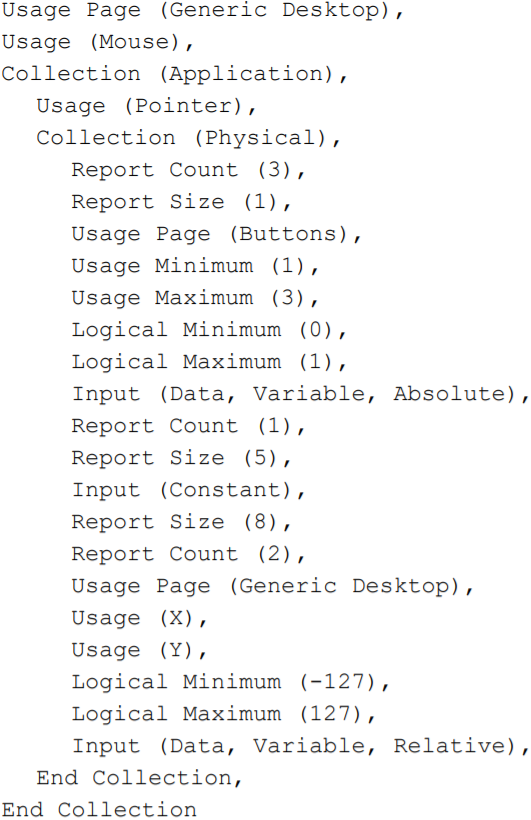
\includegraphics[width=10cm]{img/kap03_full_report_desc}
	\caption{Konkrétny príklad Report Descriptoru myši prevzatý z HID Class Specification~\cite{report_desc_mouse}}
	\label{obr:kap3:full_report_desc}
\end{figure}

\newpage

Z prvej časti (obrázok~\ref{obr:kap3:report_desc_collection}) si môžeme všimnúť, že sa celý Report Descriptor delí do logických kolekcíí -- najprv \textit{Application} a potom \textit{Physical}. Hneď na začiatku vidíme definovanú \textit{Usage Page} s hodnotou \textit{Generic Desktop}, ktorá bližšie špecifikuje nasledujúci \textit{Usage (Mouse)} item -- takže už vieme, že sa jedná o myš. 

\begin{figure}[!htb]
	\centering
	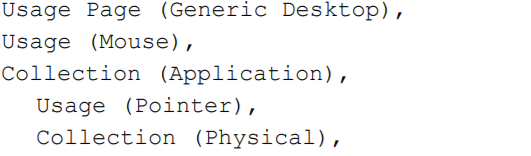
\includegraphics[width=10cm]{img/kap03_report_desc_collection}
	\caption{Časť Report Descriptoru reprezentujúca jednotlivé kolekcie}
	\label{obr:kap3:report_desc_collection}
\end{figure}

Na obrázku~\ref{obr:kap3:report_desc_buttons} vidíme ďalšiu časť descriptoru, ktorá reprezentuje tlačidlá myši -- to sme vyčítali z časti \textit{Usage Page (Buttons)}. Nasledujúce časti \textit{Report Count (3)} a \textit{Report Size (1)} nám naznačujú, že veľkosť istej podmnožiny dát budú tri 1-bitové hodnoty. Ďalej z hodnôt \textit{Logical Minimum (0)} a \textit{Logical Maximum (1)} vidíme že budú nabývať hodnoty medzi 0 a 1. Nasleduje Input item s hodnotami \textit{Data}, \textit{Variable} a \textit{Absolute} -- tie nám udávajú, že sa jedná o input zariadenia, ktorý bude modifikovateľný (hodnota \textit{Data}), budú to 3 jednotlivé 1-bitové položky (hodnota \textit{Variable}) a hodnota dát nie je relatívna voči inej hodnote (položka \textit{Absolute}). Ďalej vidíme časti \textit{Report Count (1)}, \textit{Report Size (5)} a \textit{Input (Constant)} -- Takže v inpute bude nasledovať časť o veľkosti 5 bitov, ktorá bude mať konštantnú readonly hodnotu (toto v myši väčšinou reprezentuje padding tlačidiel).

\begin{figure}[!htb]
	\centering
	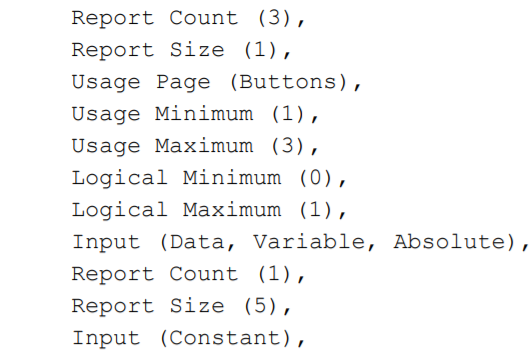
\includegraphics[width=10cm]{img/kap03_report_desc_buttons}
	\caption{Časť Report Descriptoru reprezentujúca tlačidlá myši}
	\label{obr:kap3:report_desc_buttons}
\end{figure}

Z nasledujúcej časti (obrázok~\ref{obr:kap3:report_desc_axis}) vidíme, že sa bude jednať o dve 8-bitové hodnoty (položky \textit{Report Size (8)} a \textit{Report Count (2)}). Následne sa prepne \textit{Usage Page} z \textit{Buttons} na \textit{Generic Desktop} a definujú sa 2 Usage pre \textit{X} a \textit{Y} -- tie v myši reprezentujú jednotlivé osy pohybu. Ďalej vidíme, že môžu nadobúdať hodnoty od -127 do 127 (položky \textit{Logical Minimum (-127)} a \textit{Logical Maximum (127)}) čo presne odpovedá rozsahu jedného znamienkového bytu.

\begin{figure}[!htb]
	\centering
	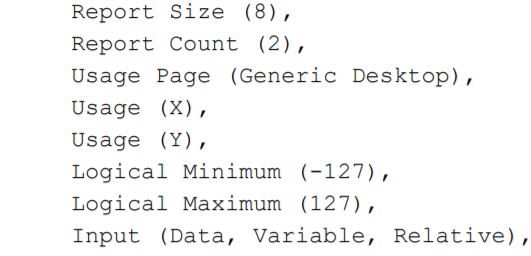
\includegraphics[width=10cm]{img/kap03_report_desc_axis}
	\caption{Časť Report Descriptoru reprezentujúca osy X a Y pri pohybe s myšou}
	\label{obr:kap3:report_desc_axis}
\end{figure}

Na poslednom obrázku~\ref{obr:kap3:report_desc_end} už len vidíme ukončenie kolekcií, čím končí aj celý Report Descriptor.

\begin{figure}[!htb]
	\centering
	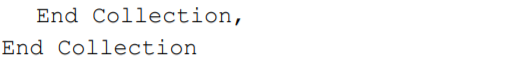
\includegraphics[width=10cm]{img/kap03_report_desc_end}
	\caption{Časť Report Descriptoru reprezentujúca ukončenie jednotlivých kolekcií}
	\label{obr:kap3:report_desc_end}
\end{figure}

V konečnom dôsledku nám z toho teda vychádza, že input našej myši bude mať veľkosť 3 byty (sčítanie všetkých \textit{Report Size} * \textit{Report Count}), kde prvé 3 bity budú reprezentovať stlačenie tlačidiel, nasledujúcich 5 bitov bude výplň a posledné 2 byty reprezentujú osy X a Y v tomto poradí. Toto reprezentuje jeden input report nášho zariadenia na jeho konkrétnom endpointe. Jeden endpoint ale môže obsahovať viac reportov (či už input, output alebo feature). V takom prípade musia byť jednotlivé reporty prefixované 1B hodnotou, ktorú nazývame \textit{Report ID} a ktorá musí byť uvedená v Report Descriptore pri jednotlivých reportoch v podobe \textit{Report ID} itemu. Ako príklad niečoho takého si môžeme predstaviť klávesnicu so zabudovaným zariadením s funkciou myši. Takáto klávesnica môže posielať informácie o stlačení kláves tak ako aj o pohybe myši v jednom endpointe. Na rozlíšenie o ktoré dáta sa jedná by sa použil Report ID.

Ostáva nám ešte jedna možnosť, ktorú sme doteraz nespomenuli -- ako priradiť Report Descriptor k jednotlivým reportom pokiaľ ich zariadenie posiela z viacerých endpointov. To si vysvetlíme v nasledujúcej sekcii.

\subsection*{Report Descriptor $\longleftrightarrow$ endpoint}
Ako už vieme z kapitoly (ODKAZ), jedno USB zariadenie môže pozostávať z viacerých interfacov. Každý interface má dané endpointy, ktoré sa s ním viažu. Pri komunikácii medzi USB hostom a zariadením si z hlavičky jednotlivých paketov vieme vytiahnuť informáciu do ktorého endpointu sa zapisujú, resp. z ktorého endpointu sa čítajú dáta. Takže v prípade reportu poslaného zariadením vieme zistiť k akému endpointu sa viaže. Hodilo by sa nám teda vedieť k jednotlivým endpointom priradiť im odpovedajúci Report Descriptor. Túto informáciu máme nepriamo poskytnutú v Setup Pakete, ktorý posiela USB host v momente keď si od zariadenia vypýta jeho Report Descriptor. Špecifikuje v ňom totiž položku \textit{wInterfaceNumber}, ktorá udáva číslo interfacu pre ktorý si USB host vypýtal Report Descriptor. Teraz nám už len stačí zistiť aké endpointy sa na daný interface viažu -- túto informáciu sme zíkali vyššie pri konfigurácii daného zariadenia, keď si USB host vypýtal od zariadenia Configuration Descriptor a spolu s ním dostal aj Interface Descriptor a jemu odpovedajúce Endpoint Descriptory.



\section{Voľba frameworku}
Pre jazyk C++ existuje hneď niekoľko známych GUI frameworkov nad ktorými sme uvažovali, ako napríklad \textit{Dear ImGui}~\cite{dearimgui}, \textit{SFGui}~\cite{sfgui} alebo \textit{Qt}~\cite{qt}. Autor tohto projektu nemal so žiadnym z týchto frameworkov predchádzajúcu skúsenosť, ale na základe rešeršu si nakoniec zvolil Qt.

\subsection*{Qt}
Qt je open-source framework na vytváranie užívateľských rozhraní. Podporuje všetky základné platformy ako Windows, Linux a macOS. Je to jeden z najznámejších a najpoužívanejších GUI frameworkov v profesionálnom prostredí medzi firmami ako napríklad LG, AMD, Panasonic, apod. To naznačuje, že sa jedná o robustný systém s rozsiahlou a dobre otestovanou funkcionalitou. Qt sa môže na prvý pohľad javiť ako zložitejši na naučenie kvôli jeho komplexnosti, na druhú stranu sa len ťažko hľadá niečo, čoho by nebol schopný. To nás dostáva k trochu špecifickému spôsobu akým sa v Qt programuje, a to je využívaním tzv. model/view architektúry~\cite{qt_model_view}.

\subsubsection*{Model/View Architektúra}
Qt obsahuje množinu itemov, ktoré používaju model/view architektúru na riadenie vzťahu medzi reprezentáciou dát a spôsobom akým sú vyobrazené. Celá architektúra vychádza zo známeho návrhového vzoru MVC~\cite{mvc} (Model-View-Controller), kde sa View a Controller zlúčia do jedného. V prípade ak chceme mierne upraviť spôsob akým viewer dáta zobrazuje (napríklad zmeniť ich farbu) použijeme na to tzv. \textit{delegate}. Architektúra sa teda dá rozdeliť do 3 hlavných komponent -- model, view a delegate. Každá z týchto komponent je definovaná abstraktnou triedou, ktoré ponúkajú jednotný interface a v niektorých prípadoch (napríklad QFileSystemModel~\cite{qfilesystemmodel}, QTableView~\cite{qtableview}, atď.) máme dokonca už predimplementovanú aj základnú funckionalitu. Komunikácia medzi komponentami prebieha pomocou tzv. \textit{signals} a \textit{slots}~\cite{signal_slot}. Signal je vyvolaný konkrétnym eventom (napríklad stlačenie tlačidla na konrétny item) a slot je funkcia, ktorá sa zavolá ako odpoveď na daný signal.

Qt má ešte jednu obrovskú výhodu, a tou je rozsiahla komunita a skvelá dokumentácia. V prípade akýchkoľvek otázok alebo nejasností sme nikdy nemali problém nájsť odpoveď, či už v spomínanej dokumentácii, alebo na rôznych užívateľských fórach.



\section{Spracovávanie pcap súborov}
Pcap je obecne známy formát súboru so špecifickým zameraním -- ukladanie dát reprezentujúcich pakety. Existuje niekoľko spôsobov ako daný súbor spracovať:

\subsection*{Npcap API}
Npcap~\cite{npcap} je Windows knižnica na zachytávanie sieťových paketov, ktorá poskytuje Npcap API~\cite{npcap_api} pomocou ktorého sme schopní spracovávať pcap súbory. Schopnosť Npcap zachytávať pakety je nám zbytočná -- jednak pretože na to využívame USBPcap a navyše Npcap je schopný zachytiť iba sieťové pakety. Jej API by nám ale mohlo zjednodušiť čítanie nami zachytených pcap súborov. Pomocou volania \texttt{pcap\_open\_offline()} získame handle pomocou ktorého môžeme neskôr čítať jednotlivé pakety volaním funkcie \texttt{pcap\_next()}, ktorá nám vráti pointer na dáta samotného paketu. Použitie je skutočne jednoduché, má to ale aj svoje nevýhody.

Za prvú nevýhodu môžeme brať nutnosť pridávať do projektu ďalšie knižnice -- čo zahŕňa inštaláciu Npcap, linkovanie dodatočných dll súborov a celkovú integráciu nášho projektu s knižnicou. Zároveň tým vytvárame akúsi závislosť nášho projektu na Npcap knižnici. Čo ale môžeme považovať za najväčšiu nevýhodu je fakt, že použitím tejto knižnice úzko viažeme náš program na platformu Windows. Windows je síce platforma na ktorú hlavne cielime, ale zároveň môžeme uvažovať nad neskôrším rozšírením na iné platformy. V takom prípade by sme museli prepísať dôležitú časť nášho kódu, ktorá by zahŕňala spracovanie pcap súborov a oddelenie dát jednotlivých paketov.

Keď sa bližšie pozrieme na formát pcap súboru, zistíme, že vôbec nie je zložitý. Celý súbor obsahuje globálnu hlavičku a dáta jednotlivých paketov sú prefixované lokálnymi hlavičkami. Preto spracovanie jednotlivých súborov nie je náročné a môžeme na to použiť bežné spôsoby.

\subsection*{QFile}
Bežný prístup k čítaniu súborov v C++ by bolo použitie \texttt{std::ifstream}~\cite{std_ifstream}, keďže ale používame Qt framework, máme k dispozícii triedu \textit{QFile}~\cite{qfile}. QFile ponúka jednoduché API vďaka ktorému môžeme postupne spracovávať ľubovoľný súbor.
Ako sme už spomínali vyššie v kapitole~\ref{kap03:third_party}, na analýzu paketov v reálnom čase používame ukladanie do súboru pomocou Wiresharku. QFile API nám umožňuje tento súbor postupne spracovávať a tým pádom sme splnili požiadavky~\ref{uvod:poz:analyza}~a~\ref{uvod:poz:analyza_real_time} ohľadom čítania súborov, ktoré sme si na začiatku stanovili.



\section{Uchovávanie informácií}
Počas spracovávania pcap súborov máme k dispozícii dáta popisujúce jednotlivé pakety. Tie si musíme určitým spôsobom zareprezentovať a ukladať, aby sme ich mohli neskôr analyzovať a vyobraziť. V tejto sekcii si rozoberieme niekoľko možných riešení.

\subsection*{char[]}
Metóda \texttt{read(char*, qint64)} pomocou ktorej čítame zo súboru špecifikuje prvým parametrom miesto do ktorého sa majú zapísať prečítané dáta a druhým parametrom akú veľkosť dát chceme prečítať. Musíme si teda dopredu pripraviť buffer do ktorého budeme zapisovať. Keďže konkrétnu veľkosť jednotlivých paketov zistíme až za run-timu, budeme musieť buffer dynamicky alokovať na halde. Na to existujú 2 hlavné spôsoby ako niečo také dosiahnuť:
\begin{itemize}
\item Pomocou \texttt{new char[paket\_size]} -- tento spôsob by sa dal v dnešnom C++ považovať za zastaralý a nebezpečný. Je nutné pečlivo sledovať životnosť takto alokovanej pamäte, musíme si na ňu držať odkaz a keď už ju nebudeme potrebovať, je potrebné na nej zavolať delete aby nám nevznikali žiadne memory leaky.
\item Pomocou \texttt{std::unique\_ptr\textless char[]\textgreater} -- tento spôsob je určite lepší ako ten predchádzajúci, pretože nám odpadá starosť o memory leaky. Na druhú stranu tu vzniká menší problém s uskladnením alebo s predávaním dát po programe v podobe parametru. Museli by sme sa starať o to, kto je vlastníkom daného objektu a či je ešte korektné ho používať.
\end{itemize}

Skúsime sa pozrieť na to, čo nám ponúka samotné Qt.

\subsection*{QByteArray}
\label{kap03:sec:uch_dat:qbytearray}
V riešení nám zase pomôže koncept dostupný v Qt -- \textit{QByteArray}~\cite{qbytearray}. QByteArray je trieda, ktorá slúži práve na uchovávanie bytov alebo '\\0'-terminated stringov. Navyše sú uložené dáta copy-on-write takže ušetríme pamäť a zbytočné kopírovanie dát. Obsahuje metódy ako \texttt{resize(int)} (zmení veľkosť daného poľa) alebo \texttt{data()} (vráti char* na začiatok poľa). O životnosť objektu sa nemusíme obávať, pretože Qt používa vlastný reference counting systém, ktorým sa stará o všetky zdieľané objekty medzi ktoré patrí aj QByteArray. O ukladaní dát sa budeme bližšie baviť v sekcii~\ref{kap03:sec:zobr_zakl} nižšie ale aby sme to pochopili, vysvetlíme si tu ešte jeden koncept Qt, ktorý neskôr využijeme spolu s QByteArray pri ukladaní dát -- \textit{QVariant}~\cite{qvariant}. QVariant je trieda, ktorá sa správa ako union pre väčšinu základných Qt datových typov. Podstatné je, že si doňho vieme zabaliť náš konkrétny QByteArray a neskôr ho odtiaľ získať zavolaním metódy \texttt{toByteArray()}.



\section{Zobrazenie základných informácií}
\label{kap03:sec:zobr_zakl}
V požiadavke~\ref{uvod:poz:zobrazenie_paketov} sme si zadefinovali aby aplikácia na prvý pohľad zobrazila len základné údaje o pakete, a detailnejšie informácie by mali byť podľa požiadavky~\ref{uvod:poz:paket_detail} zobrazené až po interakcii užívateľa. Pravdepodobne najintutívnejšia interakcia užívateľa ak chce zobraziť detailnejšie informácie je pomocou dvojkliku na konkrétnu položku. Zobrazenie základných informácií by malo byť podobné tým, aké sme mali možnosť vidieť u Wiresharku a Device Monitoring Studia v kapitole~\ref{uvod:sec:existujuce_aplikacie}. Qt nám poskytuje 2 základné triedy pomocou ktorých budeme schopní dosiahnuť podobného vzhľadu.

\subsection*{QListWidget}
QListWidget~\cite{qlistwidget} poskytuje vzhľad na základe view triedy QListView~\cite{qlistview} a jednotlivé položky sú reprezentované pomocou itemu QListWidgetItem~\cite{qlistwidgetitem}. Pomocou QListWidget sme boli schopní dosiahnuť výsledku ukázaného na obrázku~\ref{obr:kap3:ListViewLook}.

\begin{figure}[!htb]
	\centering
	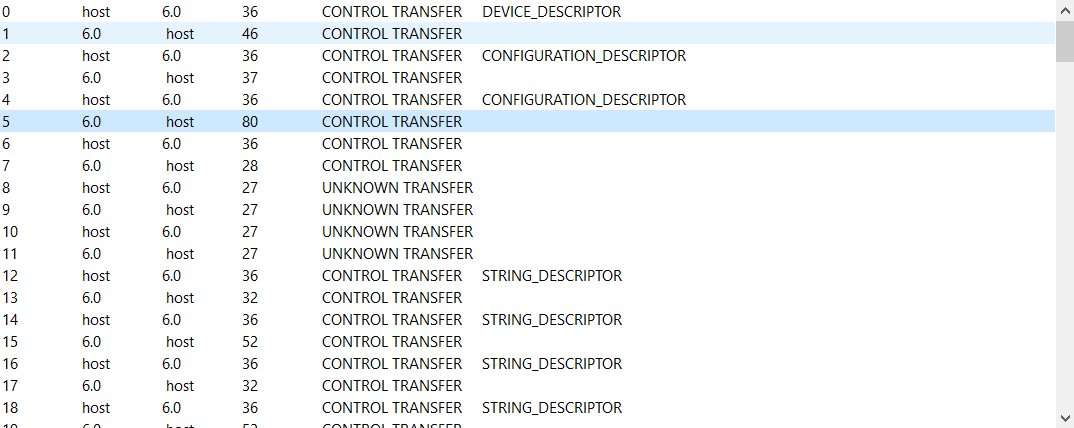
\includegraphics[width=\textwidth]{img/kap03_ListViewLook}
	\caption{Vyobrazenie základných informácií o pakete pomocou QListWidget}
	\label{obr:kap3:ListViewLook}
\end{figure}

QListWidget zároveň podporuje signal \texttt{itemDoubleClicked(QListWidgetItem*)}, ktorý má ako parameter konkrétny QListWidgetItem na ktorý užívateľ dvojklikol. Keďže chceme po dvojkliku zobraziť detailnejšie informácie o danom pakete, musíme si ich najprv niekde uschovať a následne sa k nim vedieť ľahko dostať. Tu prichádza výhoda použitia QListWidgetItem -- ten je totiž schopný si v sebe uchovať dáta v podobe QVariantu. To nám úplne vyhovuje, pretože ako sme už spomínali vyššie v sekcii~\ref{kap03:sec:uch_dat:qbytearray}, dáta si uchovávame práve v QByteArray, ktorý sme schopní zabaliť do QVariantu. Uloženie konkrétneho QVariantu je vykonané pomocou metódy \texttt{setData(int role, const QVariant \&value)} -- \texttt{role} môže byť podľa Qt dokumentácie~\cite{qitemdatarole} hodnota 256 a vyššie, druhý parameter je práve QVariant, ktorý chceme uložiť. Odkázaním sa na rovnakú \texttt{role} hodnotu v metóde \texttt{data(int role)} dostaneme ako návratovú hodnotu QVariant ktorý sme si vyššie uložili. Ďalšou výhodou je, že jeden riadok reprezentuje práve jeden QListWidgetItem, takže presne vieme v ktorom iteme máme uložené dáta.

Nevýhody sú naopak nepraktické rozšírenie o ďalšie stĺpčeky. Tým, že jeden riadok je práve jeden item, stĺpčeky sú tu len akási abstrakcia, pretože všetky informácie ktoré môžeme vidieť na obrázku~\ref{obr:kap3:ListViewLook} (napríklad index paketu na začiatku alebo typ prenosu), je len jeden dlhý string. Z toho vyplýva, že ak by sme sa v budúcnosti rozhodli rozšíriť funkcionalitu nášho programu na triedenie itemov na základe hodnoty v jednotlivých stĺpčekoch, nebolo by to možné.

\subsection*{QTableWidget}
\label{kap03:sec:table_widget}
QTableWidget~\cite{qtablewidget} poskytuje vzhľad na základe view triedy QTableView~\cite{qtableview} a jednotlivé položky sú reprezentované pomocou itemu QTableWidgetItem~\cite{qtablewidgetitem}. Pomocou QTableWidget sme dosiahli výsledok vyobrazený na obrázku~\ref{obr:kap3:TableViewLook} nižšie.

\begin{figure}[!htb]
	\centering
	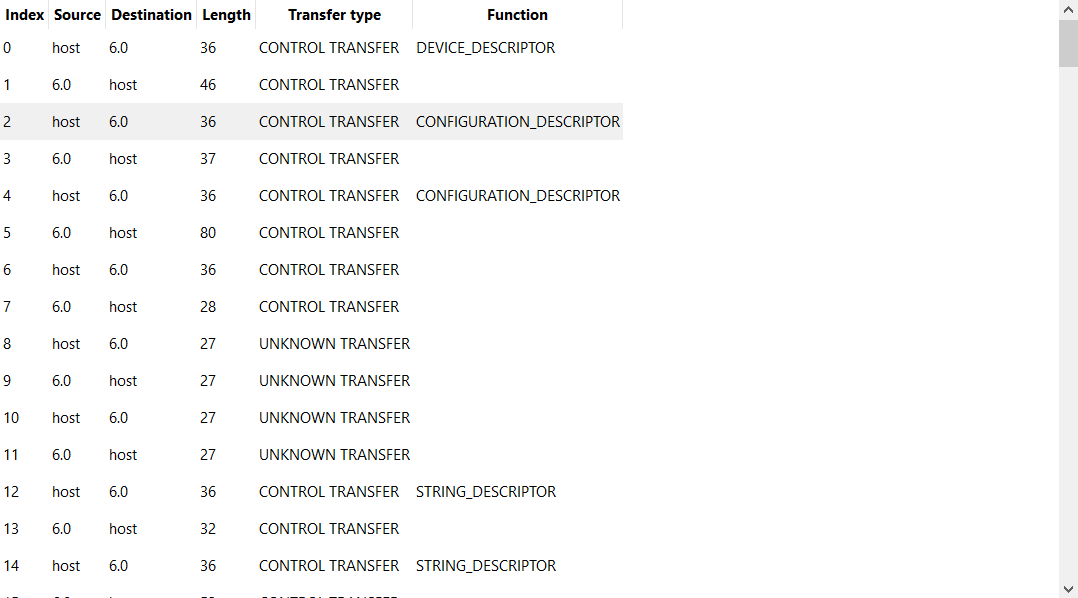
\includegraphics[width=\textwidth]{img/kap03_TableViewLook}
	\caption{Vyobrazenie základných informácií o pakete pomocou QTableWidget}
	\label{obr:kap3:TableViewLook}
\end{figure}

Ako si môžeme všimnúť, podoba medzi QListWidget a QTableWidget tak ako aj medzi QListWidgetItem a QTableWidgetItem je zrejmá, a teda nie je prekvapivé, že budú mať niektoré interné vlastnosti rovnaké. Medzi ne patria našťastie aj metódy \texttt{setData(int role, const QVariant \&value)} a \texttt{data(int role)} -- takže výhoda uchovania si dát nám ostala. QTableWidget takisto podporuje signal  \texttt{itemDoubleClicked(QTableWidgetItem*)} s rovnakými vlastnosťami ako mal QListWidget. Naopak rozdiel je napríklad v tom, že jeden riadok je teraz reprezentovaný niekoľkými QTableWidgetItemami. To nám umožňuje pridať si samotný item pre každú informáciu o pakete, ktorú chceme vyobraziť, čím zároveň vytvárame skutočné stĺpčeky. QTableWidget má zároveň možnosť pridania horizontálnej hlavičky, v ktorej vieme špecifikovať význam hodnôt v jednotlivých stĺpčekoch.

S týmito vlastnosťami nám ale vznikli aj nové problémy, ktoré musíme riešiť. Prvý problém je, že nie všetky riadky majú jednotnú dĺžku (niektoré nemajú vyplnenú hodnotu \uv{Function}, ako môžeme vidieť na obrázku~\ref{obr:kap3:TableViewLook} vyššie). To znamená, že riadok tam pôvodne nemá žiaden item -- pri dvojkliku na nevyplnenú časť by sa teda nič nestalo. Takisto pri kliknutí na riadok alebo pri vyfarbení daného riadku by bola označená resp. vyfarbená len časť v ktorej sa nachádza text -- to pôsobí nekonzistentným dojmom. Riešenie je naštastie triviálne -- v prípade, že do daného stĺpčeka nemáme čo vyplniť, vytvoríme prázdny QTableWidgetItem a ten pridáme. Ďalší problém je uchovávanie dát -- v prípade QListWidget bol jeden riadok reprezentovaný len jedným itemom, takže v prípade keď užívateľ dvojklikol na paket, ktorý chcel bližšie preskúmať, tak sme v signali \texttt{itemDoubleClicked(QListWidgetItem*)} dostali práve item v ktorom sme mali uložené všetky informácie. V prípade QTableWidget ak užívateľ dvojklikne na určitú časť riadku, zvolí sa jeden konkrétny item spomedzi všetkých na danom riadku. Problém teraz spočíva v tom, v ktorom iteme si budeme uchovávať dáta. Trochu prvoplánové riešenie by bolo ukladať si dáta do každého itemu v riadku -- toto riešenie nie je príliš ideálne, pretože vzniká zbytočná duplikácia dát. Preto si dáta uchovávame v prvom iteme každého riadku a v prípade keď užívateľ dvojklikom vyberie konkrétny item, zistíme si pomocou metódy \texttt{row(QTableWidgetItem*)} číslo riadku na ktorom sa nachádza a následne pomocou metódy \texttt{item(int row, int column)} získame prvý item v danom riadku.

V požiadavke~\ref{uvod:poz:zobrazenie_paketov} sme si takisto určili, že chceme jednotlivé pakety mať farebne oddelené na základe ich pohybu na zbernici. Túto informáciu získame z hlavičky paketu pri vytváraní jednotlivých riadkov. Rozhodli sme sa vyfarbovať riadky ktoré reprezentujú pakety posielané zariadením hostovi, pretože sa v nich väčšinou nachádzajú zaujímavejšie dáta a myslíme si, že typický užívateľ má tendenciu klikať skôr na farebne zvýraznené časti. Keďže tu nemáme jeden item reprezentujúci celý riadok, zafarbenie prebieha obyčajnou iteráciou cez všetky stĺpčeky a ich samostatným zafarbením. Celkovú funkcionalitu farebného oddelenia sme rozvinuli ešte o trochu viac oproti ostatným aplikáciám a dokonca ešte aj farba akou je item označený, sa líši na základe typu prenosu. Výsledný vzhľad môžeme vidieť na obrázku~\ref{obr:kap3:TableViewLookColor}.

\begin{figure}[!htb]
	\centering
	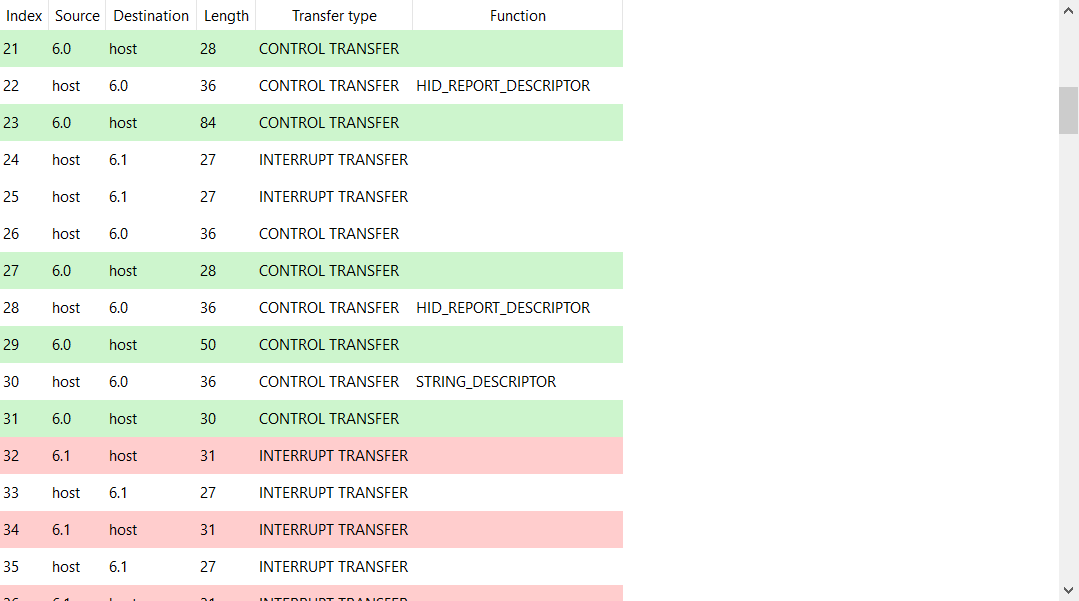
\includegraphics[width=\textwidth]{img/kap03_TableViewLookColor}
	\caption{Vyobrazenie základných informácií o pakete pomocou QTableWidget}
	\label{obr:kap3:TableViewLookColor}
\end{figure}



\section{Hexdump}
Ako sme si stanovili na začiatku v požiadavke~\ref{uvod:poz:hexdump}, chceme aby naša aplikácia bola schopná zobrazovať hexdump dát nad ktorými prebieha analýza. Chceli by sme podporovať základné správanie hexdumpu -- označením hexovej časti sa automaticky označia im odpovedajúce tlačiteľné znaky a opačne. Zároveň ale máme na náš hexdump vďaka požiadavke~\ref{uvod:poz:data_highlight} trochu väčšie nároky, a to farebné vyznačenie jednotlivých znakov podľa významu. V Qt máme 2 základné možnosti ako niečoho takého dosiahnuť -- nadefinovanie vlastného widgetu alebo prispôsobenie už existujúceho widgetu naším požiadavkám. Poďme sa teda pozrieť na to čo všetko by sme museli riešiť v prípade nadefinovania vlastného widgetu.

\subsection*{QAbstractScrollArea}
QAbstractScrollArea~\cite{qabstractscrollarea} trieda je v podstate widget, ktorý nám poskytuje abstrakciu scrollovacej plochy (scrollovanie samozrejme musíme podporovať v prípade väčšieho množstva dát). Kontent je vykresľovaný do widgetu, ktorý nazývame viewport. Dokumentácia udáva list niekoľkých vecí o ktoré sa musíme postarať ak chceme vytvoriť objekt, ktorý dedí od QAbstractScrollArea:
\begin{itemize}
\item Nastavenie scroll-barov -- to zahŕňa napríklad ich veľkosť, rozsah pohybu, definovanie o koľko sa má daný scroll-bar pohnúť v prípade ak užívateľ stlačí tlačidlo \uv{Page Up} resp. \uv{Page Down}, alebo aj sledovanie ich aktuálnej pozície.
\item Vykreslenie kontentu, ktorý sa má zobraziť na základe hodnôt jednotlivých scroll-barov (vykresliť tú časť hexdumpu na ktorej sa momentálne podľa scroll-barov nachádzame).
\item Spracovať všetky eventy, ktoré sú prijaté viewportom -- napríklad paintEvent (požaduje vykreslenie celého veiwportu alebo danej časti), mousePressEvent (kliknutie na viewport), atď.
\item Používanie \texttt{viewport->update()} k updatenutiu kontentu na viewporte namiesto \texttt{update()}.
\end{itemize}

Ako vidíme, je toho celkom dosť a preto skúsime nájsť widget, ktorý už má v Qt všetky tieto veci implementované a len ho upravíme našim požiadavkám hexdumpu.

\subsection*{QTableView}
S QTableView~\cite{qtableview} sme sa už stretli vyššie v sekcii~\ref{kap03:sec:table_widget}. Hexdump si v podstate vieme predstaviť ako tabuľku dát, preto dáva zmysel skúsiť upraviť práve túto triedu. QTableView je súčasťou Qt model/view architektúry, takže nám umožňuje logicky oddeliť dáta a ich zobrazovanie. Na reprezentáciu dát máme vytvorený vlastný model, poďme sa preto venovať len ich zobrazeniu pomocou table view. Na kompletný hexdump budeme potrebovať 2 samostatné QTableView -- jeden pre hexa časť a jeden pre tlačiteľné znaky. Pre vyobrazenie hexdumpu tak, aby sa podobal tomu na čo je bežný užívateľ zvyknutý nám postačia len jednoduché úpravy ako napríklad:

\begin{itemize}
\item Odstránenie horizontálnej hlavičky (\texttt{horizontalHeader()->setVisible(false)}).
\item Nastavenie veľkosti jednotlivých buniek (\texttt{resizeColumnsToContents()} a \texttt{resizeRowsToContents()}).
\item Odstránenie mriežky medzi bunkami (\texttt{setShowGrid(false)}).
\end{itemize}

Na implementáciu funkcionality označenia rovnakých častí tlačiteľných znakov ako hexdumpu a opačne nám stačí prepojiť signály \texttt{selectionChanged} jednotlivých selection modelov pre oba QTableView s nami definovanými funkciami (bližšie si ich opíšeme v kapitole Vývojová dokumentácia~\ref{chap:vyvoj_dok}). Keďže sa pohybujeme v model/view architektúre, na vykreslenie farebného oddelenia dát a zároveň na vyobrazenie dát samotných použijeme delegate (detailnejší popis jeho fungovania si takisto opíšeme v kapitole Vývojová dokumentácia~\ref{chap:vyvoj_dok}). Ukážku nášho výsledného hexdumpu môžeme vidieť na obrázku~\ref{obr:kap3:hexdump_color} nižšie.

\begin{figure}[!htb]
	\centering
	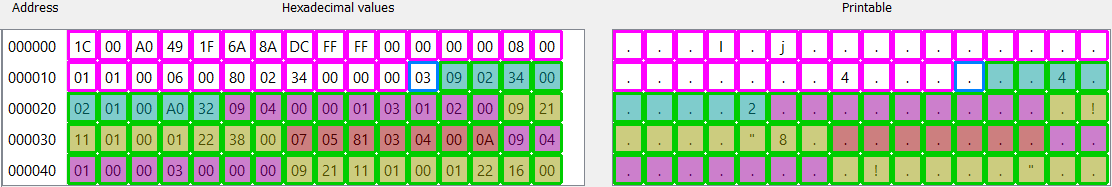
\includegraphics[width=\textwidth]{img/kap03_hexdump_color}
	\caption{Vyobrazenie hexdumpu s farebným oddelením dát podľa významu}
	\label{obr:kap3:hexdump_color}
\end{figure}

Samozrejme, obyčajné vyfarbenie nám k lepšej orientácii v hexdumpe veľmi nepomôže, pokiaľ nepoznáme význam jednotlivých farieb. Preto sme implementovali tzv. Color Map, ktorý nám k jednotlivým farbám priradí ich význam. Jej časť môžeme vidieť na obrázku~\ref{obr:kap3:color_map}.

\begin{figure}[!htb]
	\centering
	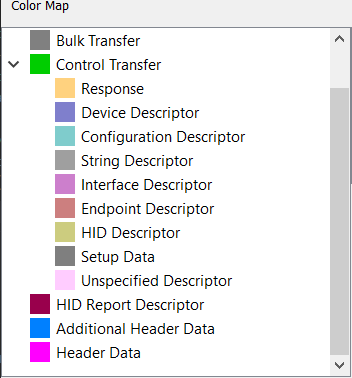
\includegraphics[width=8cm]{img/kap03_colormap}
	\caption{Časť Color Map}
	\label{obr:kap3:color_map}
\end{figure}

Takisto si uvedomujeme, že nie každému môže farebné zvýraznenie hexdumpu vyhovovať a preto dávame užívateľovi možnosť ho úplne vypnúť. Výsledok je ukázaný na obrázku~\ref{obr:kap3:hexdump_clear}.

\begin{figure}[!htb]
	\centering
	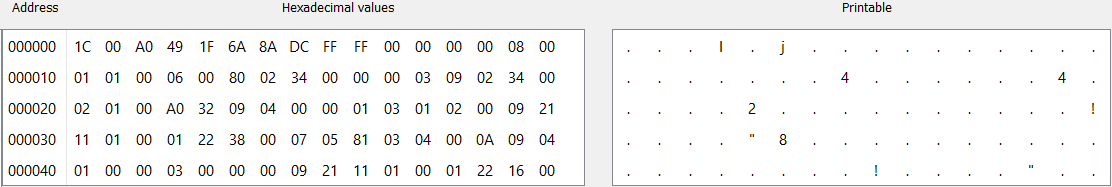
\includegraphics[width=\textwidth]{img/kap03_hexdump_clear}
	\caption{Vyobrazenie hexdumpu bez farebného oddelenia dát podľa významu}
	\label{obr:kap3:hexdump_clear}
\end{figure}

\section{Zobrazenie sémantického významu dát}
Ako sme si definovali v požiadavkách~\ref{uvod:poz:descriptory}--~\ref{uvod:poz:paket_hlavicka}, chceme byť schopní vykonávať sémenatikú analýzu pomocou stromovej štruktúry. Vzhľadom na to, že sa jedná o obecne známy spôsob vyobrazenia dát, Qt má na to špeciálnu triedu QTreeView~\cite{qtreeview}, ktorá je sučasťou Qt model/view architektúry. Takisto máme opäť možnosť nadefinovať si vlastný view pomocou dedenia od triedy \textit{QAbstractItemView}~\cite{qabstractitemview}. Ako sme už ale videli vyššie, museli by sme sami implementovať viaceré funkcionality, ktoré nám QTreeView ponúka sám a preto nevidíme dôvod nadefinovania vlastného view.

\subsection*{QTreeView}
Celkom používame až 3 QTreeView -- pre vyobrazenie hlavičky paketu, descriptorov a inputu zariadenia, a ako posledné už vyššie spomínaný Color Map. V našom konkrétnom prípade máme aj 3 odlišné modely -- jeden pre každý view. Vzhľadom na to, že sa opäť pohybujeme v Qt model/view architektúre, budeme sa teraz zaoberať iba vyobrazením dát. Keďže nám vyhovuje štandardný spôsob akým QTreeView zobrazuje svoje položky, definujeme len niekoľko základných vlastností pre jednotlivé viewery:
\begin{itemize}
\item Každému vieweru nastavíme jemu odpovedajúci model pomocou \texttt{setModel()}.
\item Nastavíme šírku jednotlivých stĺpčekov buď pomocou \texttt{resizeColumnToContents()} alebo \texttt{setColumnWidth()}.
\end{itemize}

Príklad výslednej stromovej štruktúry môžeme vidieť na obrázku~\ref{obr:kap3:tree_view}.

\begin{figure}[!htb]
	\centering
	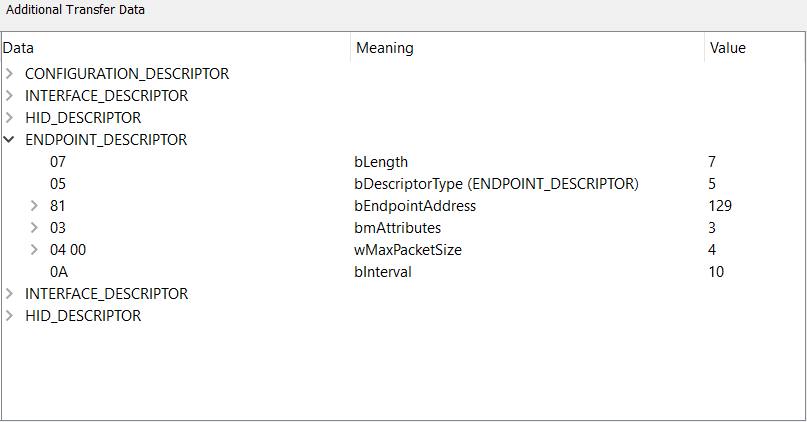
\includegraphics[width=\textwidth]{img/kap03_tree_view}
	\caption{Vyobrazenie stromovej štruktúry}
	\label{obr:kap3:tree_view}
\end{figure}